\documentclass[compress]{beamer}

%--------------------------------------------------------------------------
% Common packages
%--------------------------------------------------------------------------
\usepackage[english]{babel}
\usepackage{pgfpages} % required for notes on second screen
\usepackage{graphicx}
\usepackage{subfigure}
\usepackage{multicol}
\usepackage[normalem]{ulem}

\usepackage{tabularx,ragged2e}
\usepackage{booktabs}
\usepackage{marvosym}


\usepackage{fontawesome}
% \usepackage[tt=false, type1=true]{libertine}
% \usepackage[T1]{fontenc}



\usepackage{tikz}
\usetikzlibrary{calc,shapes,shadows}
\usetikzlibrary{fadings}
% REFERENCES
% https://tex.stackexchange.com/questions/135393/how-to-draw-bar-pie-chart
% https://tex.stackexchange.com/questions/56254/how-to-design-a-3d-donut-pie-chart-with-pgf-plot




\global\edef\lastangle{0}
\newcounter{sectornumber}


\newcommand{\ring}[4]{% angles&colors, inner, outer radius, height
\begin{scope}[x={(0.866cm,0.5cm)},y={(-0.866cm,0.5cm)},z={(0cm,1cm)}]
\global\edef\lastangle{0}
\setcounter{sectornumber}{1}
\foreach \x/\ringcolor in {#1}
{   \pgfmathsetmacro{\na}{\lastangle+\x*3.6}
    \colorlet{darkercolor}{\ringcolor!60!black}
    \colorlet{darkestcolor}{\ringcolor!20!black}
    \shadedraw[top color=darkercolor,bottom color=darkestcolor,draw=darkercolor] (\lastangle:#2) arc (\lastangle:\na:#2) -- ++(0,0,#4) arc (\na:\lastangle:#2) -- cycle;
    \shadedraw[top color=darkercolor,bottom color=darkestcolor,draw=darkercolor] (\lastangle:#3) arc (\lastangle:\na:#3) -- ++(0,0,#4) arc (\na:\lastangle:#3) -- cycle;
    \global\edef\lastangle{\na}
}
\global\edef\lastangle{0}
\foreach \x/\ringcolor in {#1}
{   \pgfmathsetmacro{\na}{\lastangle+\x*3.6}
    \colorlet{darkercolor}{\ringcolor!60!black}
    \colorlet{darkestcolor}{\ringcolor!20!black}
    \fill[\ringcolor,draw=darkercolor] (0,0,#4) ++(\lastangle:#2) arc (\lastangle:\na:#2) -- ++(\na:#3-#2) arc (\na:\lastangle:#3) -- cycle;
    \pgfmathsetmacro{\nodepos}{(#3+#2)*0.5}
    \node (n\thesectornumber) at ($(0,0,#4)+(\lastangle+\x*1.8:\nodepos)$) {};
    \stepcounter{sectornumber}
    \global\edef\lastangle{\na}
}
\end{scope}
}




\usepackage{pgfplots}

\pgfplotstableread[row sep=\\,col sep=&]{
    year & million & carD & carR \\
    2015     & 900  & 0.1  & 0.2  \\
    2030     & 1400 & 3.8  & 4.9  \\
    2050    & 2100 & 10.4 & 13.4 \\
    2100    & 3200 & 17.3 & 22.2 \\
    }\mydata






%--------------------------------------------------------------------------
% Load theme
%--------------------------------------------------------------------------
\usetheme{hri}

\usepackage{tikz}
\usetikzlibrary{patterns,shapes,fpu,fit,calc,mindmap,backgrounds,positioning,svg.path}

\tikzset{
  invisible/.style={opacity=0},
  visible on/.style={alt={#1{}{invisible}}},
  alt/.code args={<#1>#2#3}{%
    \alt<#1>{\pgfkeysalso{#2}}{\pgfkeysalso{#3}} % \pgfkeysalso doesn't change the path
  },
}

%% Neat trick to have only one navigation bullet per subsection
%% http://tex.stackexchange.com/questions/64333/one-navigation-bullet-per-subsection-with-subsection-false-in-custom-beamer-them
%\usepackage{etoolbox}
%\makeatletter
%\patchcmd{\slideentry}{\advance\beamer@xpos by1\relax}{}{}{}
%\def\beamer@subsectionentry#1#2#3#4#5{\advance\beamer@xpos by1\relax}%
%\makeatother
%%%%%%%%%%%%%%%%%%%%%%%%%%%%%%%%%%%%%%%

\graphicspath{{figs/}}

% for model of anthopomorphism
\newcommand{\IPA}{{$\mathcal{A}_0$~}}
\newcommand{\SLA}{{$\mathcal{A}_\infty$~}}
\newcommand{\sla}{{\mathcal{A}_\infty}}
\newcommand{\AntMax}{{$\mathcal{A}_{max}$~}}
\newcommand{\antMax}{{\mathcal{A}_{max}}}

% for HATP plans
\newcommand{\hatpaction}[3]{#1\\\textsf{\scriptsize #2,}\\\textsf{\scriptsize #3}}
\newcommand{\stmt}[1]{{\footnotesize \tt  #1}}

% for mutual modelling
\newcommand{\Mmodel}[3]{{\mathcal{M}(#1, #2, #3)}}
\newcommand{\model}[3]{{$\mathcal{M}(#1, #2, #3)$}}
\newcommand{\Model}[3]{{$\mathcal{M}^{\circ}(#1, #2, #3)$}}

% typeset logical concept
\newcommand{\concept}[1]{{\scriptsize \texttt{#1}}}

\newcommand{\backbutton}{\hfill\hyperlink{appendix}{\beamerreturnbutton{Supplementary material}}}




%--------------------------------------------------------------------------
% General presentation settings
%--------------------------------------------------------------------------
\title{Towards the Analysis of Human \\ Movement with  Humanoid Robots}
\subtitle{The XV Symposium of Mexican Students}
\date{Durham University -- {\bf 13 July 2017}}
\author{Miguel P. Xochicale}
\institute{Department of Electronic Engineering \\{\bf University of Birmingham}}


% \lhead{XV Symposium of Mexican Studies and Students in the United Kingdom}

%--------------------------------------------------------------------------
% Notes settings
%--------------------------------------------------------------------------
%\setbeameroption{show notes on second screen}
%\setbeameroption{hide notes}


\begin{document}


%%%%%%%%%%%%%%%%%%%%%%%%%%%%%%%%%%%%%%%%%%%%%%%%%%%%%%%%
\licenseframe{https://github.com/mxochicale/symposiummx}

%%%%%%%%%%%%%%%%%%%%%%%%%%%%%%%%%%%%%%%%%%%%%%%%%%%%%%%%
\maketitle



%--------------------------------------------------------------------------
% Content
%--------------------------------------------------------------------------
\section{Introduction}




\subsection{}
%%%%%%%%%%%%%%%%%%%%%%%%%%%%%%%%%%%%%%%%%%%%%%%%%%%%%%%%
{
\paper{ \href{http://apps.who.int/gb/ebwha/pdf_files/WHA69/A69_17-en.pdf}{A69/17, {\bf  The World Health Organization (WHO)}, April 2016  }}
\begin{frame}{The world's population is rapidly ageing}


  \normalsize
  The proportion of the world’s population aged 60 years or over will double from

  \begin{multicols}{2}


    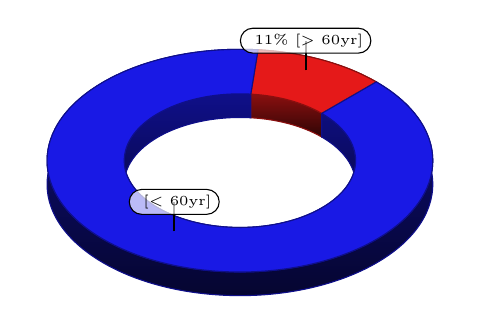
\begin{tikzpicture}
    \ring{11/red!80!gray,89/blue!80!gray}{1.2}{2}{0.3}
    \foreach \x/\label in {1/ 11\% [> 60yr], 2/ [< 60yr]}
    {   \draw[thick] (n\x) -- ++(0,0.5) node[fill=white,draw,rounded rectangle,inner sep=2pt,thin,fill opacity=0.7,text opacity=1] {\tiny\label};
    }
    \end{tikzpicture}
    \LARGE 2000

    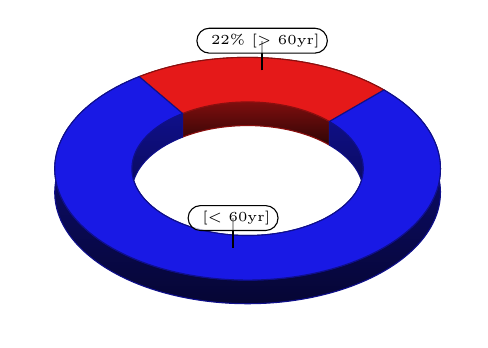
\begin{tikzpicture}
    \ring{22/red!80!gray,78/blue!80!gray}{1.2}{2}{0.3}
    \foreach \x/\label in {1/ 22\% [> 60yr] , 2/ [< 60yr]}
    {   \draw[thick] (n\x) -- ++(0,0.5) node[fill=white,draw,rounded rectangle,inner sep=2pt,thin,fill opacity=0.7,text opacity=1] {\tiny\label};
    }
    \end{tikzpicture}
    \LARGE 2050

  \end{multicols}

  \badge{/badge/xvmx_badge}
\end{frame}
}




\subsection{}
%%%%%%%%%%%%%%%%%%%%%%%%%%%%%%%%%%%%%%%%%%%%%%%%%%%%%%%%
{
\begin{frame}[plain]{}

\vspace{20mm}

        % \LARGE
        % "In 2015, 125 million people worldwide were aged 80 years or older and

        \LARGE
        By 2050 there will be almost 434 million people of 80 years or older worldwide,
        {\bf of which 80 \% will live in low- and middle-income countries}.

        % One priority area of action for a healthy ageing is the  improvement of
        % methodologies for {\bf measurement, monitoring and understanding} of
        % human movement.

        %
        %  \normalsize
        %  \~ The World Health Organization (WHO)

        % ``Cognition is a group of mental processes that includes {\bf
        % attention}, {\bf memory}, producing and understanding {\bf
        % language}, {\bf learning}, {\bf reasoning}, {\bf problem
        % solving}, and {\bf decision making}.''

        \badge{/badge/xvmx_badge}
\end{frame}
}



\subsection{}
%%%%%%%%%%%%%%%%%%%%%%%%%%%%%%%%%%%%%%%%%%%%%%%%%%%%%%%%
\imageframe[caption=]{/healthy_ageing/ah_who_H}


\subsection{}
%%%%%%%%%%%%%%%%%%%%%%%%%%%%%%%%%%%%%%%%%%%%%%%%%%%%%%%%
\imageframe[caption=]{/healthy_ageing/ah_who_R}





\section{Caring the elderly with Humanoid Robots}


\subsection{}
%%%%%%%%%%%%%%%%%%%%%%%%%%%%%%%%%%%%%%%%%%%%%%%%%%%%%%%%
{
\paper{ {\bf \href{http://www.riken.jp/en/pr/press/2011/20110802_2/}{RIKEN 2016}}  }
\begin{frame}{RI-MAN and RIBA-II robots}

  \begin{columns}


      \begin{column}{0.6\linewidth}
      \centering

          \begin{itemize}
              \item RI-MAN can track human face by integrating auditory and
              visual information.
              \item RI-MAN can do smell discernment by using semiconductor gas sensors.
              \item RIBA-II can detect a person’s weight from touch alone using
                    capacitive tactile sensors made entirely of rubber.
              \item RIBA-II can crouch down and lift a patient off a futon at floor level.
          \end{itemize}

      \end{column}


      \begin{column}{0.6\linewidth}

          \begin{figure}
              \centering
              \includegraphicscopyright[width=0.8\linewidth]{/riken/riken-robots}{Top. RI-MAN; Bottom. RIBA-II}
          \end{figure}

        \end{column}

     \end{columns}


        \badge{/badge/xvmx_badge}
\end{frame}
}


\subsection{}
%%%%%%%%%%%%%%%%%%%%%%%%%%%%%%%%%%%%%%%%%%%%%%%%%%%%%%%%
{
\paper{ {\bf \href{https://palro.jp/en/feature}{https://palro.jp/en/feature}}  }
\begin{frame}{PALRO is a Robot who cares}

  \begin{columns}


      \begin{column}{0.6\linewidth}
      \centering

          \begin{itemize}
              \item PALRO can analysis of sound types, recognise faces,
              detect moving bodies, identify individual from voice prints,
              and recognition of sound source direction.
              \item PALRO is used for recreational activities for elderly people
              that such as games, exercises, quiz and music.
          \end{itemize}

      \end{column}


      \begin{column}{0.6\linewidth}

          \begin{figure}
              \centering
              \includegraphicscopyright[width=0.8\linewidth]{/palro/figure}{}
          \end{figure}

        \end{column}

     \end{columns}

        \badge{/badge/xvmx_badge}
\end{frame}
}




\subsection{}
%%%%%%%%%%%%%%%%%%%%%%%%%%%%%%%%%%%%%%%%%%%%%%%%%%%%%%%%
{
\paper{ {\bf \href{https://www.ald.softbankrobotics.com/en/cool-robots/nao/find-out-more-about-nao}{NAO by Aldebaran}}  }
\begin{frame}{NAO (a humanoid robot)}



          \begin{figure}
              \centering
              \includegraphicscopyright[width=0.9\linewidth]{/nao/nao}{NAO has 25 degrees of freedom, capacitive sensors, sonars,
              4 mics, speakers, 2 cameras, internet access.}
          \end{figure}

        \badge{/badge/xvmx_badge}
\end{frame}
}



\subsection{}
%%%%%%%%%%%%%%%%%%%%%%%%%%%%%%%%%%%%%%%%%%%%%%%%%%%%%%%%
{
\paper{ {\bf \href{https://www.youtube.com/channel/UCbT8GS9L_IdYvpCeNRd2gVg}{(A,C) Zora Robots}; \href{https://www.swinburne.edu.au/science-engineering-technology/staff/profile/index.php?id=cdmccarthy}{(B) McCarthy et al. 2016}; \href{https://www.youtube.com/watch?v=77a20MzLVwQ}{(D) NAOTherapist}  }  }
\begin{frame}{NAO as a Physiotherapist}

  \begin{figure}
      \centering
      \includegraphicscopyright[width=0.9\linewidth]{/nao/applications}{}
  \end{figure}


        \badge{/badge/xvmx_badge}
\end{frame}
}


\subsection{}
%%%%%%%%%%%%%%%%%%%%%%%%%%%%%%%%%%%%%%%%%%%%%%%%%%%%%%%%
{
\paper{ {\bf  \href{https://www.youtube.com/watch?v=Ys2iCoivTBk}{Robocoach by Ngee Ann Polytechnic in Singapore}   }  }
\begin{frame}{Robocoach}

          \begin{figure}
              \centering
              \includegraphicscopyright[width=0.9\linewidth]{/robocoach/robocoach}{Robocoach coaches the elderly to perform 15 types of arm exercise.}
          \end{figure}

        \badge{/badge/xvmx_badge}
\end{frame}
}


\section{Methods and Results}


\subsection{}
%%%%%%%%%%%%%%%%%%%%%%%%%%%%%%%%%%%%%%%%%%%%%%%%%%%%%%%%
{
\paper{   \href{https://github.com/mxochicale/publications/tree/master/2017/HRI}{MP Xochicale et al., {\bf Towards the Quantification of Human-Robot Interaction Using Wearable Inertial Sensors}, 2017  }  }
\begin{frame}{Human-Robot Imitation}

          \begin{figure}
              \centering
              \includegraphicscopyright[width=0.8\linewidth]{/hri17/figA}{Horizontal Arm Movement of a Front to Front Human-Robot Imitation.}
          \end{figure}

        \badge{/badge/xvmx_badge}
\end{frame}
}


\subsection{}
%%%%%%%%%%%%%%%%%%%%%%%%%%%%%%%%%%%%%%%%%%%%%%%%%%%%%%%%
{
% \paper{   \href{https://github.com/mxochicale/publications/tree/master/2017/HRI}{MP Xochicale et al., {\bf Towards the Quantification of Human-Robot Interaction Using Wearable Inertial Sensors}, 2017  }  }
\begin{frame}{Human Activity Recognition Chain}

          \begin{figure}
              \centering
              \includegraphicscopyright[width=1.0\linewidth]{/har/fig_harc}{}
          \end{figure}

        \badge{/badge/xvmx_badge}
\end{frame}
}


\subsection{}
%%%%%%%%%%%%%%%%%%%%%%%%%%%%%%%%%%%%%%%%%%%%%%%%%%%%%%%%
{
\paper{   \href{https://github.com/mxochicale/publications/tree/master/2017/HRI}{MP Xochicale et al., {\bf Towards the Quantification of Human-Robot Interaction Using Wearable Inertial Sensors}, 2017  }  }
\begin{frame}{Human-Robot Imitation}

          \begin{figure}
              \centering
              \includegraphicscopyright[width=0.4\linewidth]{/hri17/figDG}{Different erros for robot and participants}
          \end{figure}

        \badge{/badge/xvmx_badge}
\end{frame}
}






\section{Conclusions and Future Work}


\subsection{}
%%%%%%%%%%%%%%%%%%%%%%%%%%%%%%%%%%%%%%%%%%%%%%%%%%%%%%%%
{
\begin{frame}{Conclusions}


          \begin{itemize}
              \item It has been proposed a metric based on the Euclidean distances
              in the state space to quantify how close a participant imitate NAO's movement.
              \item (+) The state space provide a good representation of the
              variability of the activities.
              \item (-) The quality of the metric is debatable and needs further
              investigation.
          \end{itemize}

        \badge{/badge/xvmx_badge}
\end{frame}
}

\subsection{}
%%%%%%%%%%%%%%%%%%%%%%%%%%%%%%%%%%%%%%%%%%%%%%%%%%%%%%%%
{
\begin{frame}{Future Research Goals}

  Exploration of complex movements which can be performed by both
  persons and NAO.

          \begin{figure}
              \centering
              \includegraphicscopyright[width=1.0\linewidth]{/human-e-motion_setup/he_setup}{From Motion to Motion and Emotion}
          \end{figure}

        \badge{/badge/xvmx_badge}
\end{frame}
}


\subsection{}
%%%%%%%%%%%%%%%%%%%%%%%%%%%%%%%%%%%%%%%%%%%%%%%%%%%%%%%%
{
\begin{frame}{Future Research Goals}

  Exploration of Deep Neural Networks for automatic \\
  classification of people's motions and facial expressions.

          \begin{figure}
              \centering
              \includegraphicscopyright[width=0.76\linewidth]{/human-e-motion/he}{From Motion to Motion and Emotion}
          \end{figure}

        \badge{/badge/xvmx_badge}
\end{frame}
}




\section{}



% %%%%%%%%%%%%%%%%%%%%%%%%%%%%%%%%%%%%%%%%%%%%%%%%%%%%%%%%
% {
%     \fullbackground[color=black]{eeg-headset}
%
% \begin{frame}[plain]
%
%     \vspace{8cm}
%
% \setbeamercolor{hriSec1Demo}{fg=white!70!black}
%
% \begin{beamercolorbox}[wd=\linewidth,ht=6ex,dp=0.7ex]{hriSec1Demo}
%     \textbf{Gracias }\\
%     \scriptsize
%     Miguel P. Xochicale\\
%     {\tt \href{http://mxochicale.github.io/}{[http://mxochicale.github.io/]}  }
%     \href{https://twitter.com/_mxochicale}{[\faTwitter@\_mxochicale]}
%     \href{https://github.com/mxochicale}{[\faGithub@mxochicale]}
% \end{beamercolorbox}
%     \vfill
% \end{frame}
% }



%%%%%%%%%%%%%%%%%%%%%%%%%%%%%%%%%%%%%%%%%%%%%%%%%%%%%%%%
\closingtitle


%%%%%%%%%%%%%%%%%%%%%%%%%%%%%%%%%%%%%%%%%%%%%%%%%%%%%%%%
\begin{frame}{Bibliography}
    \begin{thebibliography}{10}

\beamertemplatearticlebibitems
  \bibitem{Oppenheim2009}
      M. P. Xochicale, C. Baber and M. Oussalah
      \newblock \doublequoted{Towards Quantification of Human-Robot Interaction Using Wearable Inertial Sensors}
      \newblock 12nd Conference of Human-Robot Interaction (HRI2017) March 2017, Vienna, Austria. [\href{https:// github.com/mxochicale/publications/tree/master/2017/HRI}{\faGithub}]

\beamertemplatearticlebibitems
  \bibitem{Comotti2014}
      D. Comotti, M. Galizzi, and A. Vitali
      \newblock \doublequoted{NeMEMSi: One step forward in wireless attitude and heading reference systems}
      \newblock 1st IEEE International Symposium on Inertial Sensors and Systems, 2014


    \end{thebibliography}
\end{frame}



%%%%%%%%%%%%%%%%%%%%%%%%%%%%%%%%%%%%%%%%%%%%%%%%%%%%%%%%
\licenseframe{https://github.com/mxochicale/symposiummx}





\end{document}
